% CS631A Advanced Programming in the UNIX Environment
% Author: Jan Schaumann <jschauma@netmeister.org>
% $Id: slides.tex,v 1.3 2005/10/25 20:47:04 jschauma Exp $
\special{! TeXDict begin /landplus90{true}store end }

\documentclass[xga]{xdvislides}
\usepackage[landscape]{geometry}
\usepackage{graphics}
\usepackage{graphicx}
\usepackage{colordvi}

\begin{document}
\setfontphv

%%% Headers and footers
\lhead{\slidetitle}
\chead{CS631 - Advanced Programming in the UNIX Environment}
\rhead{Slide \thepage}
\lfoot{\Gray{Lecture 08: Advanced I/O: Nonblocking I/O, I/O Multiplexing and Record Locking}}
\cfoot{\relax}
\rfoot{\Gray{\today}}

\vspace*{\fill}
\begin{center}
	\Hugesize
		CS631 - Advanced Programming in the UNIX Environment\\
		-- \\
		Advanced I/O / HTTP \\
	\hspace*{5mm}\blueline\\ [1em]
	\Normalsize
		Department of Computer Science\\
		Stevens Institute of Technology\\
		Jan Schaumann\\
		\verb+jschauma@stevens.edu+\\
		\verb+http://www.cs.stevens.edu/~jschauma/631/+
\end{center}
\vspace*{\fill}

\subsection{Nonblocking I/O}
Recall from our lecture on signals that certain system calls can block forever:
\begin{itemize}
	\item {\tt read(2)} from a particular file, if data isn't present (pipes,
		terminals, network devices)
	\item {\tt write(2)} to the same kind of file
	\item {\tt open(2)} of a particular file until a specific condition occurs
	\item {\tt read(2)} and {\tt write(2)} of files that have mandatory
		locking enabled
	\item certain {\tt ioctls(2)}
	\item some IPC functions (such as {\tt sendto(2)} or {\tt recv(2)})
\end{itemize}
\vspace{.25in}
See {\tt eintr.c} from that lecture.

\subsection{Nonblocking I/O}
Recall from our lecture on signals that certain system calls can block forever:
\begin{itemize}
	\item {\tt read(2)} from a particular file, if data isn't present (pipes,
		terminals, network devices)
	\item {\tt write(2)} to the same kind of file
	\item {\tt open(2)} of a particular file until a specific condition occurs
	\item {\tt read(2)} and {\tt write(2)} of files that have mandatory
		locking enabled
	\item certain {\tt ioctls(2)}
	\item some IPC functions (such as {\tt sendto(2)} or {\tt recv(2)})
\end{itemize}
\vspace{.25in}
Nonblocking I/O lets us issue an I/O operation and not have it block forever.
If the operation cannot be completed, return is made immediately with an error
noting that the operating would have blocked ({\tt EWOULDBLOCK} or {\tt EAGAIN}).

\subsection{Nonblocking I/O}
Ways to specify nonblocking mode:
\begin{itemize}
	\item pass {\tt O\_NONBLOCK} to {\tt open(2)}: \\

		{\tt open({\em path}, O\_RDRW|O\_NONBLOCK);}
		\vspace{.2in}
	\item set {\tt O\_NONBLOCK} via {\tt fcntl(2)}: \\

		{\tt flags = fcntl({\em fd}, F\_GETFL, 0); \\
		     fcntl({\em fd}, F\_SETFL, flags|O\_NONBLOCK);}
\end{itemize}

\subsection{Nonblocking I/O}
\begin{verbatim}
$ cc -Wall nonblock.c
$ ./a.out >/dev/null
wrote 100000 bytes
[...]
$ ./a.out | ( sleep 3; cat >/dev/null ) 2>&1 | more
[...]
$ ( ./a.out | cat >/dev/null ) 2>&1 | more
[...]
write error: Resource temporarily unavailable
wrote 3392 bytes
wrote 65536 bytes
write error: Resource temporarily unavailable
[...]
$ nc -l 8080

$ ./a.out | nc hostname 8080
[...]
\end{verbatim}

\subsection{Resource Locking}
Ways we have learned so far to ensure only one process has exclusive
access to a resource:
\begin{itemize}
	\item open file using {\tt O\_CREAT|O\_EXCL}, then immediately
		{\tt unlink(2)} it
	\item create a ``lockfile'' -- if file exists, somebody else is
		using the resource
	\item use of a semaphore
\end{itemize}

What are some problems with each of these?

\subsection{Advisory Locking}
\small
\setlength{\unitlength}{1mm}
\begin{center}
	\begin{picture}(150,22)
		\thinlines
		\put(0,0){\framebox(130,22){}}
		\put(10,17){{\tt \#include <fcntl.h>}}
		\put(10,10){{\tt int flock(int {\em fd},int {\em operation});}}
		\put(80,3){Returns: 0 if OK, -1 otherwise}
	\end{picture}
\end{center}
\Normalsize
\begin{itemize}
	\item applies or removes an advisory lock on the file associated with
		the file descriptor fd
	\item {\em operation} can be {\tt LOCK\_NB} and any one of:
		\begin{itemize}
			\item {\tt LOCK\_SH}
			\item {\tt LOCK\_EX}
			\item {\tt LOCK\_UN}
		\end{itemize}
	\item locks entire file
\end{itemize}

\subsection{Advisory Locking}
\begin{verbatim}
$ cc -Wall flock.c
1$ ./a.out
Shared lock established - sleeping for 10 seconds.
[...]
Giving up all locks.

2$ ./a.out
Shared lock established - sleeping for 10 seconds.
Now trying to get an exclusive lock.
Unable to get an exclusive lock.
[...]
Exclusive lock established.

1$ ./a.out
[blocks until the other process terminates]


\end{verbatim}

\subsection{Advisory ``Record'' Locking}
Record locking is done using {\tt fcntl(2)}, using one of {\tt F\_GETLK}, {\tt
F\_SETLK} or {\tt F\_SETLKW} and passing a
\begin{verbatim}
struct flock {
    short l_type;   /* F_RDLCK, F_WRLCK, or F_UNLCK */
    off_t l_start;  /* offset in bytes from l_whence */
    short l_whence; /* SEEK_SET, SEEK_CUR, or SEEK_END */
    off_t l_len;    /* length, in bytes; 0 means "lock to EOF" */
    pid_t l_pid;    /* returned by F_GETLK */
}
\end{verbatim}
Lock types are:
\begin{itemize}
	\item {\tt F\_RDLCK} -- Non-exclusive (read) lock; fails if write lock exists.
	\item {\tt F\_WRLCK} -- Exclusive (write) lock; fails if any lock exists.
	\item {\tt F\_UNLCK} -- Releases our lock on specified range.
\end{itemize}


\subsection{Advisory ``Record'' locking}
\small
\setlength{\unitlength}{1mm}
\begin{center}
	\begin{picture}(180,20)
		\thinlines
		\put(0,0){\framebox(160,20){}}
		\put(10,15){{\tt \#include <unistd.h>}}
		\put(10,7){{\tt int lockf(int {\em fd}, int {\em value}, off\_t {\em size});}}
		\put(100,3){Returns: 0 on success, -1 on error}
	\end{picture}
\end{center}
\Normalsize

{\em value} can be:
\begin{itemize}
	\item {\tt F\_ULOCK} -- unlock locked sections
	\item {\tt F\_LOCK} -- lock a section for exclusive use
	\item {\tt F\_TLOCK} -- test and lock a section for exclusive use
	\item {\tt F\_TEST} -- test a section for locks by other processes
\end{itemize}
\begin{center}
	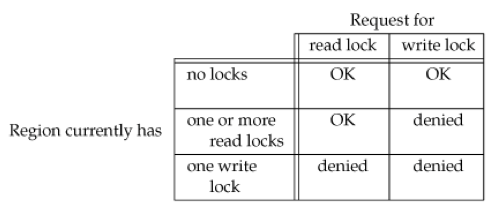
\includegraphics[angle=-90,scale=0.7]{pics/locking.eps}
\end{center}

\subsection{Advisory ``Record'' locking}
Locks are:
\begin{itemize}
	\item released if a process terminates
	\item released if a filedescriptor is closed (!)
	\item not inherited across {\tt fork(2)}
	\item inherited across {\tt exec(2)}
	\item released upon {\tt exec(2)} if close-on-exec is set
\end{itemize}

\subsection{Advisory ``Record'' locking}
Locks are associated with a {\em file and process pair}, not with a {\em filedescriptor}!
\begin{verbatim}
fd1 = open(pathname, ...);
write_lock(fd1...);        /* lock byte 0 */
if ((pid = fork()) > 0) {
        fd2 = dup(fd1);
        fd3 = open(pathname, ...);
} else if (pid == 0) {
        read_lock(fd1...); /* lock byte 1 */
}
\end{verbatim}

\subsection{Advisory ``Record'' locking}
Locks are associated with a {\em file and process pair}, not with a {\em filedescriptor}!
\begin{center}
	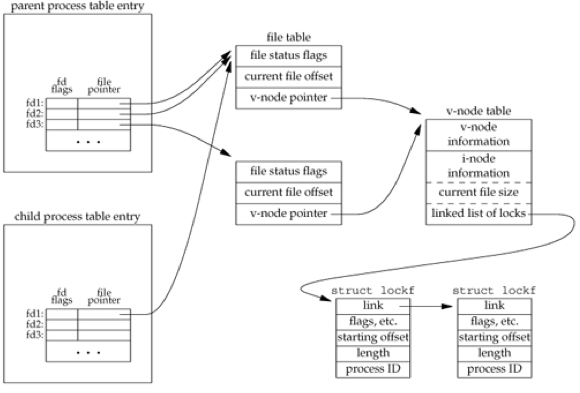
\includegraphics[angle=-90,scale=0.8]{pics/locking-structures.eps}
\end{center}

\subsection{Mandatory locking}
\begin{itemize}
	\item not implemented on all UNIX flavors
		\begin{itemize}
			\item {\tt chmod g+s,g-x file}
		\end{itemize}
	\item possible to be circumvented:
\end{itemize}
\begin{verbatim}
$ mandatory-lock /tmp/file &
$ echo foo > /tmp/file2
$ rm /tmp/file
$ mv /tmp/file2 /tmp/file
\end{verbatim}

\subsection{I/O Multiplexing}
Standard I/O loop:
\begin{verbatim}
while ((n = read(fd1, buf, BUFFSIZE)) > 0) {
        if (write(fd2, buf, n) != n) {
                fprintf(stderr, "write error\n");
                exit(1);
         }
}
\end{verbatim}

Suppose you want to read from multiple file descriptors - now what?



\subsection{I/O Multiplexing}
When handling I/O on multiple file descriptors, we have the following
options:

\begin{itemize}
	\item blocking mode: open one fd, block, wait (possibly forever),
		then test the next fd
	\item fork and use one process for each, communicate using signals
		or other IPC
	\item non-blocking mode: open one fd, immediately get results,
		open next fd, immediately get results, sleep for some time
	\item asynchronous I/O: get notified by the kernel when either fd
		is ready for I/O
\end{itemize}

\subsection{I/O Multiplexing}
Instead of blocking forever (undesirable), using {\em non-blocking} mode
(busy-polling is inefficient) or using {\em asynchronous I/O} (somewhat
limited), we can:
\begin{itemize}
	\item build a set of file descriptors we're interested in
	\item call a function that will return if any of the file
		descriptors are ready for I/O (or a timeout has elapsed)
\end{itemize}

\subsection{I/O Multiplexing}
\small
\setlength{\unitlength}{1mm}
\begin{center}
	\begin{picture}(180,40)
		\thinlines
		\put(0,0){\framebox(160,40){}}
		\put(10,35){{\tt \#include <sys/types.h>}}
		\put(10,30){{\tt \#include <sys/time.h>}}
		\put(10,25){{\tt \#include <unistd.h>}}
		\put(10,18){{\tt int select(int {\em maxfdp1}, fd\_set *{\em readfds}, fd\_set *{\em writefds}}}
		\put(40,13){{\tt fd\_set *{\em exceptfds}, struct timeval *{\em tvptr});}}
		\put(60,5){Returns: count of ready descriptors, 0 on timeout, -1 otherwise}
	\end{picture}
\end{center}
\Normalsize
Arguments passed:
\begin{itemize}
	\item which descriptors we're interested in
	\item what conditions we're interested in
	\item how long we want to wait
		\begin{itemize}
			\item {\tt tvptr == NULL} means wait forever
			\item {\tt tvptr->tv\_sec == tvptr->tv\_usec == 0} means don't wait at all
			\item wait for specified amount of time
		\end{itemize}
\end{itemize}
\vspace{.25in}
{\tt select(2)} tells us both the total count of descriptors that are
ready as well as which ones are ready.


\subsection{I/O Multiplexing}
\begin{itemize}
	\item filedescriptor sets are manipulated using the {\tt FD\_*} functions/macros
	\item read/write sets indicate readiness for read/write; {\em except} indicates an exception condition (for example OOB data, certain terminal events)
	\item EOF means ready for read - {\tt read(2)} will just return 0 (as usual)
	\item {\tt pselect(2)} provides finer-grained timeout control;
allows you to specify a signal mask (original signal mask is restored
upon return)
	\item {\tt poll(2)} provides a conceptually similar interface
\end{itemize}
\vspace{.5in}
See also:
\begin{itemize}
	\item last week's {\tt strchkread.c}
	\item \verb+http://daniel.haxx.se/docs/poll-vs-select.html+
\end{itemize}

\subsection{Asynchronous I/O}
\begin{itemize}
	\item System V derived async I/O
		\begin{itemize}
			\item limited to STREAMS
			\item enabled via {\tt ioctl(2)}
			\item uses {\tt SIGPOLL}
		\end{itemize}
	\item BSD derived async I/O
		\begin{itemize}
			\item limited to terminals and networks
			\item enabled via {\tt fcntl(2)} ({\tt O\_ASYNC},
{\tt  F\_SETOWN})
			\item uses {\tt SIGIO} and {\tt SIGURG}
		\end{itemize}
\end{itemize}
\addvspace{.5in}
Mentioned here for completeness's sake only.

See {\tt aio(7)} for an example of POSIX AIO.


\subsection{Memory Mapped I/O}
\small
\setlength{\unitlength}{1mm}
\begin{center}
	\begin{picture}(180,30)
		\thinlines
		\put(0,0){\framebox(160,30){}}
		\put(10,25){{\tt \#include <sys/types.h>}}
		\put(10,20){{\tt \#include <sys/mman.h>}}
		\put(10,12){{\tt void *mmap(void *{\em addr}, size\_t {\em len}, int {\em prot}, int {\em flags}, int {\em fd}, off\_t {\em offset});}}
		\put(95,3){Returns: pointer to mapped region if OK}
	\end{picture}
\end{center}
\Normalsize
Protection specified for a region:
\begin{itemize}
	\item {\tt PROT\_READ} -- region can be read
	\item {\tt PROT\_WRITE} -- region can be written
	\item {\tt PROT\_EXEC} -- region can be executed
	\item {\tt PROT\_NONE} -- region can not be accessed
\end{itemize}
\vspace{.25in}
{\em flag} needs to be one of
\begin{itemize}
	\item {\tt MAP\_SHARED}
	\item {\tt MAP\_PRIVATE}
	\item {\tt MAP\_COPY}
\end{itemize}
which may be OR'd with other flags (see {\tt mmap(2)} for details).

\subsection{Memory Mapped I/O}
\begin{center}
	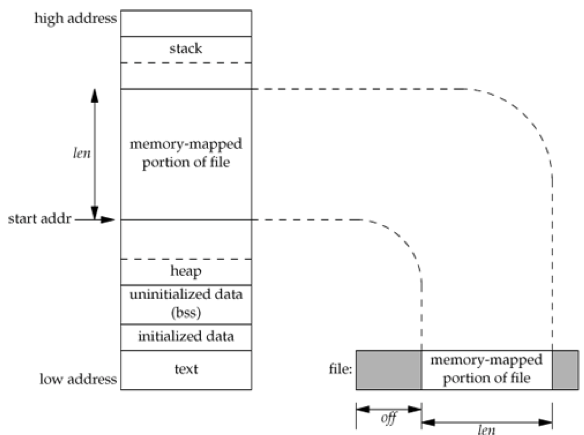
\includegraphics[angle=-90,scale=0.8]{pics/mmap.eps}
\end{center}

\subsection{Memory Mapped I/O}
\begin{center}
	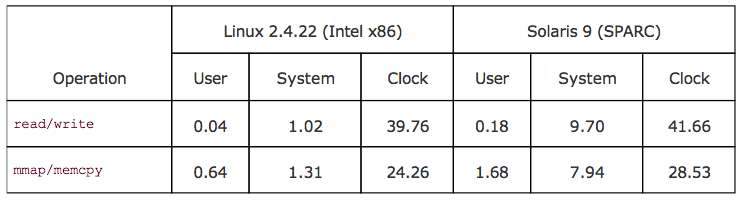
\includegraphics[angle=-90,scale=0.8]{pics/mmap-timing.eps}
\end{center}
\addvspace{.5in}
Exercise: write a program that benchmarks this performance and run it on
the systems you have access to.

\subsection{Memory Mapped I/O}
\\
\vspace*{\fill}
\verb+http://cvsweb.netbsd.org/bsdweb.cgi/src/bin/cp/utils.c?rev=HEAD+
\vspace*{\fill}

\subsection{Final Project}
\\
\vspace*{\fill}
Final project: write a simple web server. \\
{\tt http://www.cs.stevens.edu/\~{}jschauma/631/f13-final-project.html}
\vspace*{\fill}

\subsection{HTTP}
\vspace{.5in}
\begin{center}
	\Huge
	Hypertext Transfer Protocol
	\\
	\vspace{.5in}
	RFC2616
\end{center}
\Normalsize

\subsection{HTTP}
\vspace{.5in}
\begin{center}
	\Huge
	HTTP is a request/response protocol.
\end{center}
\Normalsize

\subsection{The Hypertext Transfer Protocol}
HTTP is a request/response protocol:
\begin{enumerate}
	\item client sends a request to the server
	\item server responds
\end{enumerate}

\subsection{The Hypertext Transfer Protocol}
HTTP is a request/response protocol:
\begin{enumerate}
	\item client sends a request to the server
		\begin{itemize}
			\item request method
			\item URI
			\item protocol version
			\item request modifiers
			\item client information
		\end{itemize}
	\item server responds
\end{enumerate}

\subsection{HTTP: A client request}
\vspace*{.5in}
\\
\Hugesize
\begin{center}
\begin{verbatim}
$ telnet www.google.com 80
Trying 2607:f8b0:400c:c02::93...
Connected to www.google.com.
Escape character is '^]'.
GET / HTTP/1.0

\end{verbatim}
\end{center}
\Normalsize
\vspace*{\fill}


\subsection{The Hypertext Transfer Protocol}
HTTP is a request/response protocol:
\begin{enumerate}
	\item client sends a request to the server
		\begin{itemize}
			\item request method
			\item URI
			\item protocol version
			\item request modifiers
			\item client information
		\end{itemize}
	\item server responds
		\begin{itemize}
			\item status line (including success or error code)
			\item server information
			\item entity metainformation
			\item content
		\end{itemize}
\end{enumerate}

\subsection{HTTP: a server response}
%\newcommand{\smallish}{\fontsize{18}{18}\selectfont}
%\smallish
\begin{verbatim}
HTTP/1.0 200 OK
Date: Mon, 22 Oct 2012 03:08:18 GMT
Content-Type: text/html; charset=ISO-8859-1
Server: gws

<!doctype html><html itemscope="itemscope"
itemtype="http://schema.org/WebPage"><head><meta content="Search the
world's information, including webpages, images, videos and more. Google
has many special features to help you find exactly what you're looking
for." name="description"><meta content="noodp" name="robots"><meta
itemprop="image"
content="/images/google_favicon_128.png"><title>Google</title><script>
window.google={kEI:"oriEUNmMGMX50gH6kYGwBw",getEI:function(a){var
b;while(a&&!(a.getAttribute&&(b=a.getAttribute("eid"))))a=a.parentNode;return
b||google.kEI},https:function(){return
window.location.protocol=="https:"},kEXPI:"25657,30316,39523,39977,40362
\end{verbatim}
%\Normalsize

\subsection{The Hypertext Transfer Protocol}
Server status codes:
\begin{itemize}
	\item {\bf 1xx} -- Informational; Request received, continuing process
	\item {\bf 2xx} -- Success; The action was successfully received,
        understood, and accepted
	\item {\bf 3xx} -- Redirection; Further action must be taken in order to
        complete the request
	\item {\bf 4xx} -- Client Error; The request contains bad syntax or
		cannot be fulfilled
	\item {\bf 5xx} -- Server Error; The server failed to fulfill an
		apparently valid request
\end{itemize}

\subsection{HTTP: A client request}
\newcommand{\smallish}{\fontsize{16}{16}\selectfont}
\smallish
\begin{center}
\begin{verbatim}
$ telnet www.cs.stevens.edu 80
Trying 155.246.89.84...
Connected to tarantula.srcit.stevens-tech.edu.
Escape character is '^]'.
GET / HTTP/1.0

HTTP/1.1 200 OK
Date: Mon, 04 Apr 2011 02:16:14 GMT
Server: Apache/2.2.9 (Debian) DAV/2 SVN/1.5.1 PHP/5.2.6-1+lenny9 with Suhosin-Patch mod_ssl/2.2.9 OpenSSL/0.9.8o
Last-Modified: Wed, 17 Nov 2010 19:25:54 GMT
Content-Type: text/html

<!DOCTYPE HTML PUBLIC "-//W3C//DTD HTML 4.0 Transitional//EN">
<html>
<head>
<title>SRCIT wiki page</title>
<meta http-equiv="REFRESH"
content="0;url=http://www.srcit.stevens.edu/wiki"></HEAD>
<BODY>
</BODY>
</HTML>
\end{verbatim}
\end{center}
\Normalsize

\subsection{HTTP - more than just text}
HTTP is a {\em Transfer Protocol} -- serving {\em data}, not any specific
text format.

\begin{itemize}
	\item {\tt Accept-Encoding} client header can specify different formats
		such as {\em gzip}, {\em Shared Dictionary Compression over HTTP (SDCH)} etc.
	\item corresponding server headers: {\tt Content-Type} and
		{\tt Content-Encoding}
\end{itemize}
\begin{center}
	
\includegraphics[scale=0.6,angle=-90]{pics/datatransfer.eps}
\end{center}

\subsection{HTTP - more than just static data}
HTTP is a {\em Transfer Protocol} -- what is transferred need not be
static; resources may generate different data to return based on many
variables.

\begin{itemize}
	\item CGI -- resource is {\em executed}, needs to generate
		appropriate response headers
	\item server-side scripting (ASP, PHP, Perl, ...)
	\item client-side scripting (JavaScript/ECMAScript/JScript,...)
	\item applications based on HTTP, using:
		\begin{itemize}
			\item AJAX
			\item RESTful services
			\item JSON, XML, YAML to represent state and
				abstract information
		\end{itemize}
\end{itemize}

\subsection{Writing a {\em simple} HTTP server}
\begin{itemize}
	\item parse command-line options, initialize world, ...
	\item open socket
	\item run as a d\ae mon, loop forever
		\begin{itemize}
			\item accept connection
			\item fork child to handle request
		\end{itemize}
	\item upon {\tt SIGHUP} re-read configuration, restart
\end{itemize}

\subsection{Writing a {\em simple} HTTP server}
Processing requests consists of:
\begin{itemize}
	\item reading request from socket
	\item parsing request
		\begin{itemize}
			\item valid syntax?
			\item type of request (GET, HEAD, POST)?
			\item determine pathname
				\begin{itemize}
					\item $\sim$ translation
					\item translate relative into absolute pathname
				\end{itemize}
		\end{itemize}
	\item generate server status response
	\item handle request
\end{itemize}

\subsection{Writing a {\em simple} HTTP server}
Processing requests consists of:
\begin{itemize}
	\item handling regular file request
		\begin{itemize}
			\item {\tt stat(2)} file
			\item {\tt open(2)} file
			\item {\tt read(2)} file
			\item {\tt write(2)} to socket
			\item {\tt close(2)} file
			\item terminate connection
			\item exit child handler
		\end{itemize}
	\item handling CGI execution
		\begin{itemize}
			\item setup environment
			\item setup filedescriptors (stdin/stdout)
			\item fork-exec executable
		\end{itemize}
\end{itemize}

\subsection{Homework}
Be able to explain how the shell executes the following statement: \\
{\tt ( ./a.out | cat >/dev/null ) 2>\&1 | more}

\vspace{.5in}
HW\#3: webserver framework \\
{\tt http://www.cs.stevens.edu/\~{}jschauma/631/f13-hw3.html}

\vspace{.5in}
Final project: write a simple web server. \\
{\tt http://www.cs.stevens.edu/\~{}jschauma/631/f13-final-project.html}

\end{document}
